% Options for packages loaded elsewhere
\PassOptionsToPackage{unicode}{hyperref}
\PassOptionsToPackage{hyphens}{url}
%
\documentclass[
]{article}
\usepackage{amsmath,amssymb}
\usepackage{lmodern}
\usepackage{ifxetex,ifluatex}
\ifnum 0\ifxetex 1\fi\ifluatex 1\fi=0 % if pdftex
  \usepackage[T1]{fontenc}
  \usepackage[utf8]{inputenc}
  \usepackage{textcomp} % provide euro and other symbols
\else % if luatex or xetex
  \usepackage{unicode-math}
  \defaultfontfeatures{Scale=MatchLowercase}
  \defaultfontfeatures[\rmfamily]{Ligatures=TeX,Scale=1}
\fi
% Use upquote if available, for straight quotes in verbatim environments
\IfFileExists{upquote.sty}{\usepackage{upquote}}{}
\IfFileExists{microtype.sty}{% use microtype if available
  \usepackage[]{microtype}
  \UseMicrotypeSet[protrusion]{basicmath} % disable protrusion for tt fonts
}{}
\makeatletter
\@ifundefined{KOMAClassName}{% if non-KOMA class
  \IfFileExists{parskip.sty}{%
    \usepackage{parskip}
  }{% else
    \setlength{\parindent}{0pt}
    \setlength{\parskip}{6pt plus 2pt minus 1pt}}
}{% if KOMA class
  \KOMAoptions{parskip=half}}
\makeatother
\usepackage{xcolor}
\IfFileExists{xurl.sty}{\usepackage{xurl}}{} % add URL line breaks if available
\IfFileExists{bookmark.sty}{\usepackage{bookmark}}{\usepackage{hyperref}}
\hypersetup{
  pdftitle={Networks1 rmd},
  hidelinks,
  pdfcreator={LaTeX via pandoc}}
\urlstyle{same} % disable monospaced font for URLs
\usepackage[margin=1in]{geometry}
\usepackage{color}
\usepackage{fancyvrb}
\newcommand{\VerbBar}{|}
\newcommand{\VERB}{\Verb[commandchars=\\\{\}]}
\DefineVerbatimEnvironment{Highlighting}{Verbatim}{commandchars=\\\{\}}
% Add ',fontsize=\small' for more characters per line
\usepackage{framed}
\definecolor{shadecolor}{RGB}{248,248,248}
\newenvironment{Shaded}{\begin{snugshade}}{\end{snugshade}}
\newcommand{\AlertTok}[1]{\textcolor[rgb]{0.94,0.16,0.16}{#1}}
\newcommand{\AnnotationTok}[1]{\textcolor[rgb]{0.56,0.35,0.01}{\textbf{\textit{#1}}}}
\newcommand{\AttributeTok}[1]{\textcolor[rgb]{0.77,0.63,0.00}{#1}}
\newcommand{\BaseNTok}[1]{\textcolor[rgb]{0.00,0.00,0.81}{#1}}
\newcommand{\BuiltInTok}[1]{#1}
\newcommand{\CharTok}[1]{\textcolor[rgb]{0.31,0.60,0.02}{#1}}
\newcommand{\CommentTok}[1]{\textcolor[rgb]{0.56,0.35,0.01}{\textit{#1}}}
\newcommand{\CommentVarTok}[1]{\textcolor[rgb]{0.56,0.35,0.01}{\textbf{\textit{#1}}}}
\newcommand{\ConstantTok}[1]{\textcolor[rgb]{0.00,0.00,0.00}{#1}}
\newcommand{\ControlFlowTok}[1]{\textcolor[rgb]{0.13,0.29,0.53}{\textbf{#1}}}
\newcommand{\DataTypeTok}[1]{\textcolor[rgb]{0.13,0.29,0.53}{#1}}
\newcommand{\DecValTok}[1]{\textcolor[rgb]{0.00,0.00,0.81}{#1}}
\newcommand{\DocumentationTok}[1]{\textcolor[rgb]{0.56,0.35,0.01}{\textbf{\textit{#1}}}}
\newcommand{\ErrorTok}[1]{\textcolor[rgb]{0.64,0.00,0.00}{\textbf{#1}}}
\newcommand{\ExtensionTok}[1]{#1}
\newcommand{\FloatTok}[1]{\textcolor[rgb]{0.00,0.00,0.81}{#1}}
\newcommand{\FunctionTok}[1]{\textcolor[rgb]{0.00,0.00,0.00}{#1}}
\newcommand{\ImportTok}[1]{#1}
\newcommand{\InformationTok}[1]{\textcolor[rgb]{0.56,0.35,0.01}{\textbf{\textit{#1}}}}
\newcommand{\KeywordTok}[1]{\textcolor[rgb]{0.13,0.29,0.53}{\textbf{#1}}}
\newcommand{\NormalTok}[1]{#1}
\newcommand{\OperatorTok}[1]{\textcolor[rgb]{0.81,0.36,0.00}{\textbf{#1}}}
\newcommand{\OtherTok}[1]{\textcolor[rgb]{0.56,0.35,0.01}{#1}}
\newcommand{\PreprocessorTok}[1]{\textcolor[rgb]{0.56,0.35,0.01}{\textit{#1}}}
\newcommand{\RegionMarkerTok}[1]{#1}
\newcommand{\SpecialCharTok}[1]{\textcolor[rgb]{0.00,0.00,0.00}{#1}}
\newcommand{\SpecialStringTok}[1]{\textcolor[rgb]{0.31,0.60,0.02}{#1}}
\newcommand{\StringTok}[1]{\textcolor[rgb]{0.31,0.60,0.02}{#1}}
\newcommand{\VariableTok}[1]{\textcolor[rgb]{0.00,0.00,0.00}{#1}}
\newcommand{\VerbatimStringTok}[1]{\textcolor[rgb]{0.31,0.60,0.02}{#1}}
\newcommand{\WarningTok}[1]{\textcolor[rgb]{0.56,0.35,0.01}{\textbf{\textit{#1}}}}
\usepackage{graphicx}
\makeatletter
\def\maxwidth{\ifdim\Gin@nat@width>\linewidth\linewidth\else\Gin@nat@width\fi}
\def\maxheight{\ifdim\Gin@nat@height>\textheight\textheight\else\Gin@nat@height\fi}
\makeatother
% Scale images if necessary, so that they will not overflow the page
% margins by default, and it is still possible to overwrite the defaults
% using explicit options in \includegraphics[width, height, ...]{}
\setkeys{Gin}{width=\maxwidth,height=\maxheight,keepaspectratio}
% Set default figure placement to htbp
\makeatletter
\def\fps@figure{htbp}
\makeatother
\setlength{\emergencystretch}{3em} % prevent overfull lines
\providecommand{\tightlist}{%
  \setlength{\itemsep}{0pt}\setlength{\parskip}{0pt}}
\setcounter{secnumdepth}{-\maxdimen} % remove section numbering
\ifluatex
  \usepackage{selnolig}  % disable illegal ligatures
\fi

\title{Networks1 rmd}
\author{}
\date{\vspace{-2.5em}}

\begin{document}
\maketitle

\hypertarget{r-markdown}{%
\subsection{R Markdown}\label{r-markdown}}

This is an R Markdown document. Markdown is a simple formatting syntax
for authoring HTML, PDF, and MS Word documents. For more details on
using R Markdown see \url{http://rmarkdown.rstudio.com}.

When you click the \textbf{Knit} button a document will be generated
that includes both content as well as the output of any embedded R code
chunks within the document. You can embed an R code chunk like this:

\begin{Shaded}
\begin{Highlighting}[]
\FunctionTok{summary}\NormalTok{(cars)}
\end{Highlighting}
\end{Shaded}

\begin{verbatim}
##      speed           dist       
##  Min.   : 4.0   Min.   :  2.00  
##  1st Qu.:12.0   1st Qu.: 26.00  
##  Median :15.0   Median : 36.00  
##  Mean   :15.4   Mean   : 42.98  
##  3rd Qu.:19.0   3rd Qu.: 56.00  
##  Max.   :25.0   Max.   :120.00
\end{verbatim}

\hypertarget{including-plots}{%
\subsection{Including Plots}\label{including-plots}}

You can also embed plots, for example:

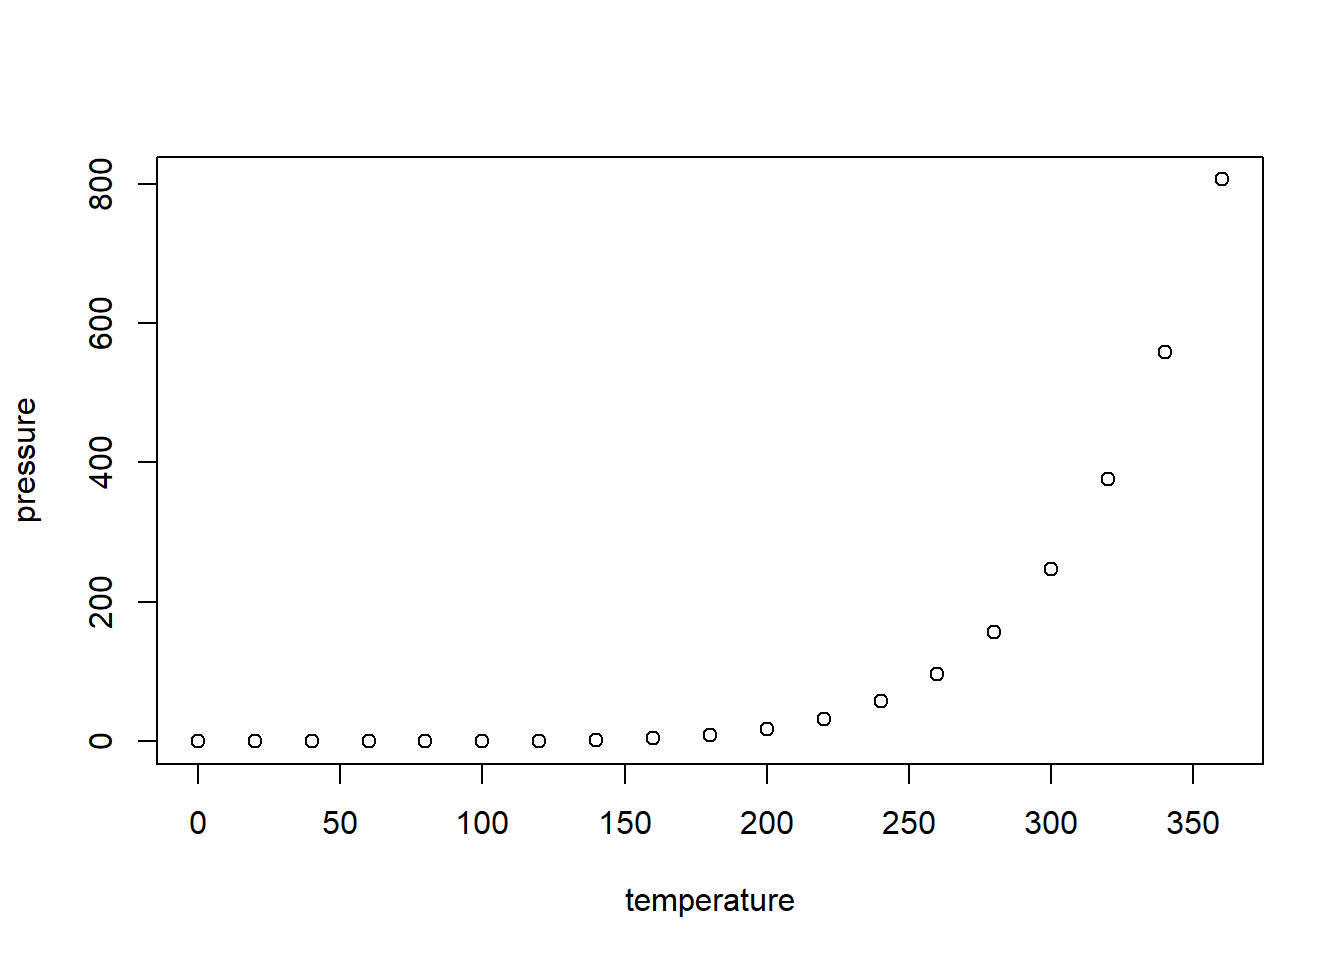
\includegraphics{Networks1_files/figure-latex/pressure-1.pdf}

Note that the \texttt{echo\ =\ FALSE} parameter was added to the code
chunk to prevent printing of the R code that generated the plot.

\begin{Shaded}
\begin{Highlighting}[]
\FunctionTok{options}\NormalTok{(}\AttributeTok{java.parameters =} \StringTok{"{-}Xmx2G"}\NormalTok{)}

\FunctionTok{library}\NormalTok{(r5r)}
\end{Highlighting}
\end{Shaded}

\begin{verbatim}
## Loading required namespace: sf
\end{verbatim}

\begin{verbatim}
## Loading required namespace: rJava
\end{verbatim}

\begin{verbatim}
## Please make sure you have already allocated some memory to Java by running:
##   options(java.parameters = '-Xmx2G').
## Currently, Java memory is set to -Xmx2G
\end{verbatim}

\begin{Shaded}
\begin{Highlighting}[]
\FunctionTok{library}\NormalTok{(osmextract)}
\end{Highlighting}
\end{Shaded}

\begin{verbatim}
## Data (c) OpenStreetMap contributors, ODbL 1.0. https://www.openstreetmap.org/copyright.
## Check the package website, https://docs.ropensci.org/osmextract/, for more details.
\end{verbatim}

\begin{Shaded}
\begin{Highlighting}[]
\FunctionTok{library}\NormalTok{(tidyverse)}
\end{Highlighting}
\end{Shaded}

\begin{verbatim}
## -- Attaching packages --------------------------------------- tidyverse 1.3.1 --
\end{verbatim}

\begin{verbatim}
## v ggplot2 3.3.5     v purrr   0.3.4
## v tibble  3.1.4     v dplyr   1.0.7
## v tidyr   1.1.3     v stringr 1.4.0
## v readr   2.0.1     v forcats 0.5.1
\end{verbatim}

\begin{verbatim}
## -- Conflicts ------------------------------------------ tidyverse_conflicts() --
## x dplyr::filter() masks stats::filter()
## x dplyr::lag()    masks stats::lag()
\end{verbatim}

\begin{Shaded}
\begin{Highlighting}[]
\FunctionTok{library}\NormalTok{(sf)}
\end{Highlighting}
\end{Shaded}

\begin{verbatim}
## Linking to GEOS 3.9.0, GDAL 3.2.1, PROJ 7.2.1
\end{verbatim}

\begin{Shaded}
\begin{Highlighting}[]
\FunctionTok{library}\NormalTok{(ggthemes)}
\FunctionTok{library}\NormalTok{(ggspatial)}
\FunctionTok{library}\NormalTok{(tigris)}
\end{Highlighting}
\end{Shaded}

\begin{verbatim}
## To enable 
## caching of data, set `options(tigris_use_cache = TRUE)` in your R script or .Rprofile.
\end{verbatim}

\begin{Shaded}
\begin{Highlighting}[]
\FunctionTok{library}\NormalTok{(wesanderson)}
\FunctionTok{library}\NormalTok{(tidytransit)}
\end{Highlighting}
\end{Shaded}

\begin{Shaded}
\begin{Highlighting}[]
\FunctionTok{dir.create}\NormalTok{(}\StringTok{"networks"}\NormalTok{)}
\end{Highlighting}
\end{Shaded}

\begin{verbatim}
## Warning in dir.create("networks"): 'networks' already exists
\end{verbatim}

\begin{Shaded}
\begin{Highlighting}[]
\FunctionTok{download.file}\NormalTok{(}\StringTok{"https://transitfeeds.com/p/wmata/75/latest/download"}\NormalTok{, }\FunctionTok{file.path}\NormalTok{(}\StringTok{"networks"}\NormalTok{,}\StringTok{"DCgtfs.zip"}\NormalTok{), }\AttributeTok{mode =} \StringTok{"wb"}\NormalTok{, }\AttributeTok{quiet=}\ConstantTok{TRUE}\NormalTok{)}
\end{Highlighting}
\end{Shaded}

\begin{Shaded}
\begin{Highlighting}[]
\NormalTok{DC\_file }\OtherTok{\textless{}{-}} \FunctionTok{oe\_match}\NormalTok{(}\StringTok{"Washington, District of Columbia"}\NormalTok{)}
\end{Highlighting}
\end{Shaded}

\begin{verbatim}
## No exact match found for place = Washington, District of Columbia and provider = geofabrik. Best match is us/district-of-columbia. 
## Checking the other providers.
\end{verbatim}

\begin{verbatim}
## No exact match found in any OSM provider data. Searching for the location online.
\end{verbatim}

\begin{verbatim}
## The input place was matched with us/district-of-columbia.
\end{verbatim}

\begin{Shaded}
\begin{Highlighting}[]
\NormalTok{DC\_streets }\OtherTok{\textless{}{-}} \FunctionTok{oe\_read}\NormalTok{(DC\_file}\SpecialCharTok{$}\NormalTok{url, }
                   \AttributeTok{provider =} \StringTok{"openstreetmap\_fr"}\NormalTok{, }
                   \AttributeTok{download\_directory =} \StringTok{"networks"}\NormalTok{, }
                   \AttributeTok{layer =} \StringTok{"lines"}\NormalTok{, }
                   \AttributeTok{quiet =} \ConstantTok{TRUE}\NormalTok{) }\SpecialCharTok{\%\textgreater{}\%}
  \FunctionTok{filter}\NormalTok{(}\SpecialCharTok{!}\FunctionTok{is.na}\NormalTok{(highway)) }
\end{Highlighting}
\end{Shaded}

\#\#\#Hello!!!\#\#\#

\begin{Shaded}
\begin{Highlighting}[]
\FunctionTok{ggplot}\NormalTok{(DC\_streets) }\SpecialCharTok{+}
  \FunctionTok{geom\_sf}\NormalTok{()}
\end{Highlighting}
\end{Shaded}

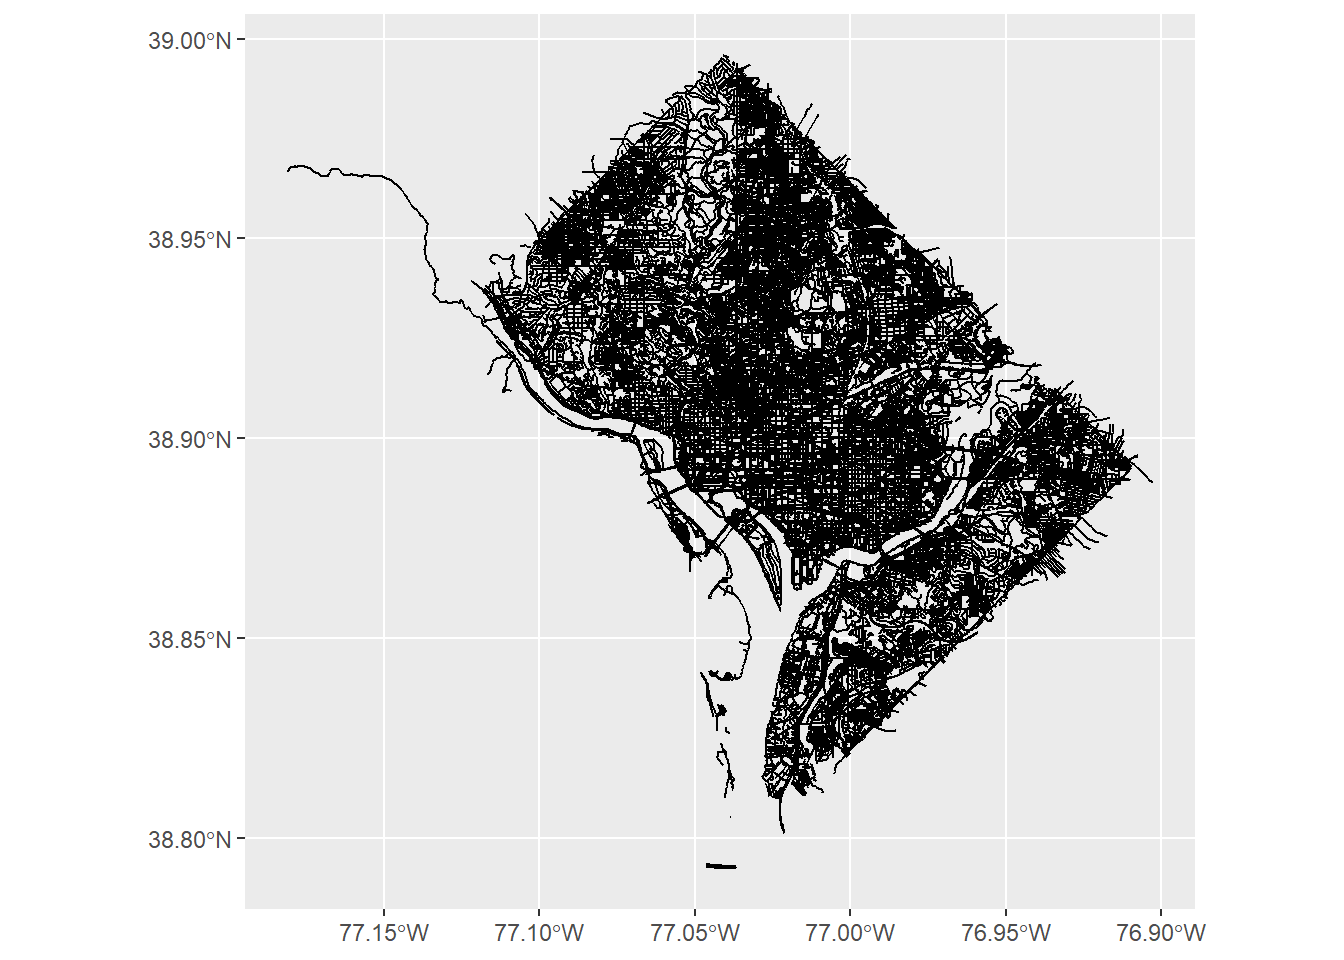
\includegraphics{Networks1_files/figure-latex/unnamed-chunk-5-1.pdf}

\begin{Shaded}
\begin{Highlighting}[]
\NormalTok{MD\_state\_plane }\OtherTok{\textless{}{-}} \StringTok{"+proj=lcc +lat\_1=39.45 +lat\_2=38.3 +lat\_0=37.66666666666666 +lon\_0={-}77 +x\_0=399999.9998983998 +y\_0=0 +ellps=GRS80 +datum=NAD83 +to\_meter=0.3048006096012192 +no\_defs"}

\NormalTok{DC\_city\_limits }\OtherTok{\textless{}{-}} \FunctionTok{places}\NormalTok{(}\StringTok{"District of Columbia"}\NormalTok{) }\SpecialCharTok{\%\textgreater{}\%}
  \FunctionTok{filter}\NormalTok{(NAME }\SpecialCharTok{==} \StringTok{"Washington"}\NormalTok{) }\SpecialCharTok{\%\textgreater{}\%}
  \FunctionTok{st\_transform}\NormalTok{(}\AttributeTok{crs =} \FunctionTok{st\_crs}\NormalTok{(DC\_streets))}
\end{Highlighting}
\end{Shaded}

\begin{verbatim}
##   |                                                                              |                                                                      |   0%  |                                                                              |=============                                                         |  19%  |                                                                              |=============================                                         |  42%  |                                                                              |=====================================================                 |  76%  |                                                                              |======================================================================| 100%
\end{verbatim}

\begin{Shaded}
\begin{Highlighting}[]
\NormalTok{DC\_streets }\OtherTok{\textless{}{-}}\NormalTok{ DC\_streets[DC\_city\_limits,]}

\FunctionTok{ggplot}\NormalTok{(DC\_streets) }\SpecialCharTok{+}
  \FunctionTok{geom\_sf}\NormalTok{() }\SpecialCharTok{+}
  \FunctionTok{coord\_sf}\NormalTok{(}\AttributeTok{crs =}\NormalTok{ MD\_state\_plane) }
\end{Highlighting}
\end{Shaded}

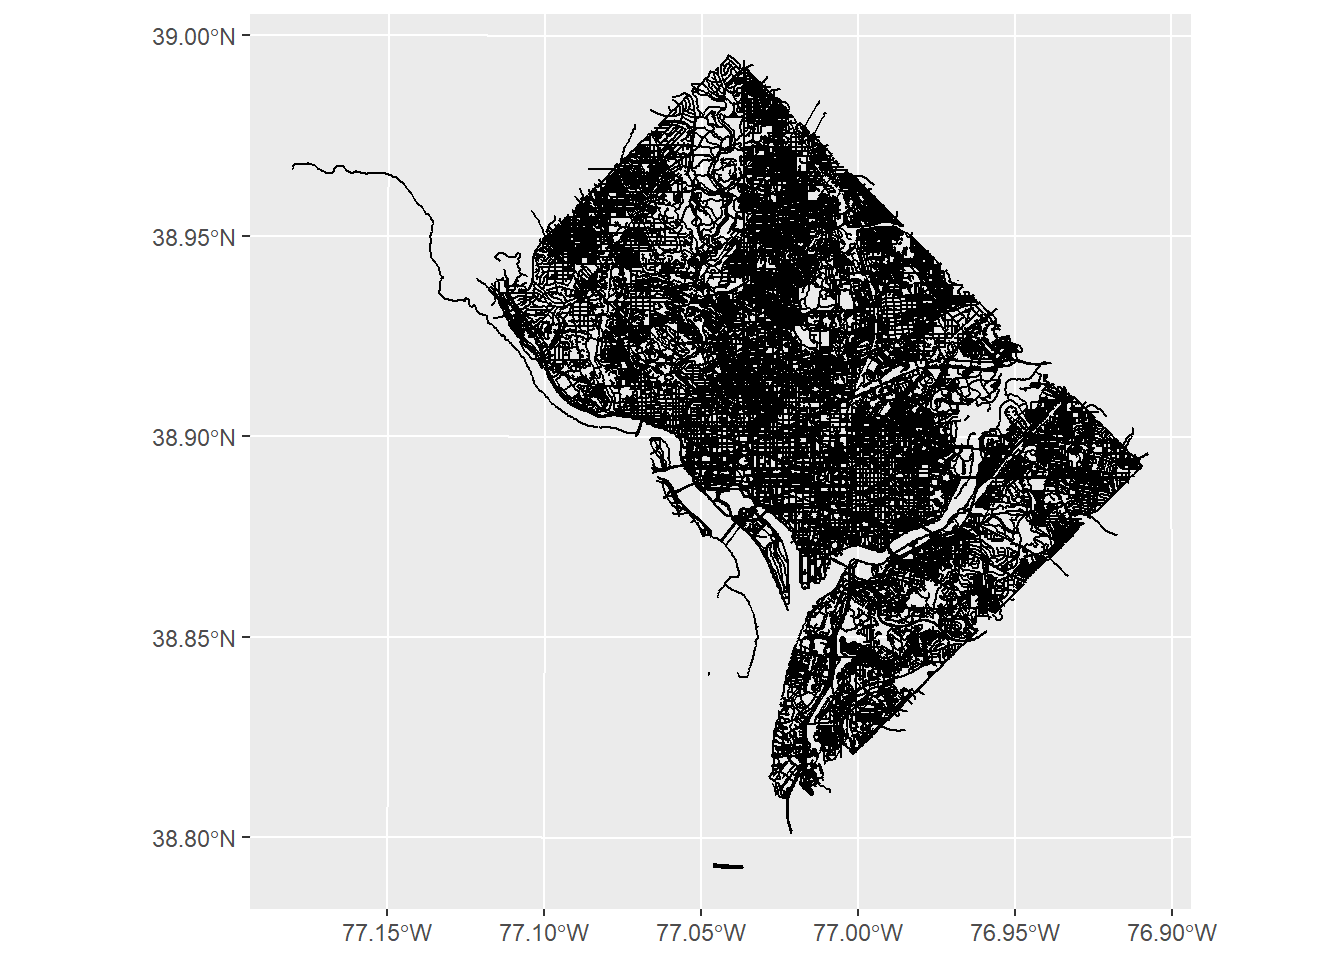
\includegraphics{Networks1_files/figure-latex/unnamed-chunk-6-1.pdf}

\begin{Shaded}
\begin{Highlighting}[]
\NormalTok{DC\_libraries }\OtherTok{\textless{}{-}} \FunctionTok{oe\_read}\NormalTok{(DC\_file}\SpecialCharTok{$}\NormalTok{url, }
                   \AttributeTok{provider =} \StringTok{"openstreetmap\_fr"}\NormalTok{, }
                   \AttributeTok{download\_directory =} \StringTok{"networks"}\NormalTok{, }
                   \AttributeTok{layer =} \StringTok{"points"}\NormalTok{, }
                   \AttributeTok{quiet =} \ConstantTok{TRUE}\NormalTok{) }\SpecialCharTok{\%\textgreater{}\%}
  \FunctionTok{filter}\NormalTok{(}\FunctionTok{str\_detect}\NormalTok{(other\_tags, }\StringTok{\textquotesingle{}"amenity"=\textgreater{}"library"\textquotesingle{}}\NormalTok{)) }\SpecialCharTok{\%\textgreater{}\%}
  \FunctionTok{st\_filter}\NormalTok{(DC\_city\_limits) }\SpecialCharTok{\%\textgreater{}\%}
  \FunctionTok{rename}\NormalTok{(}\AttributeTok{id =}\NormalTok{ osm\_id)}

\FunctionTok{ggplot}\NormalTok{(DC\_streets) }\SpecialCharTok{+}
  \FunctionTok{geom\_sf}\NormalTok{(}\AttributeTok{color =} \StringTok{\textquotesingle{}gray\textquotesingle{}}\NormalTok{) }\SpecialCharTok{+}
  \FunctionTok{geom\_sf}\NormalTok{(}\AttributeTok{data =}\NormalTok{ DC\_libraries, }\AttributeTok{color =} \StringTok{"darkblue"}\NormalTok{) }\SpecialCharTok{+}
  \FunctionTok{coord\_sf}\NormalTok{(}\AttributeTok{crs =}\NormalTok{ MD\_state\_plane)  }\SpecialCharTok{+}
  \FunctionTok{theme\_void}\NormalTok{()}
\end{Highlighting}
\end{Shaded}

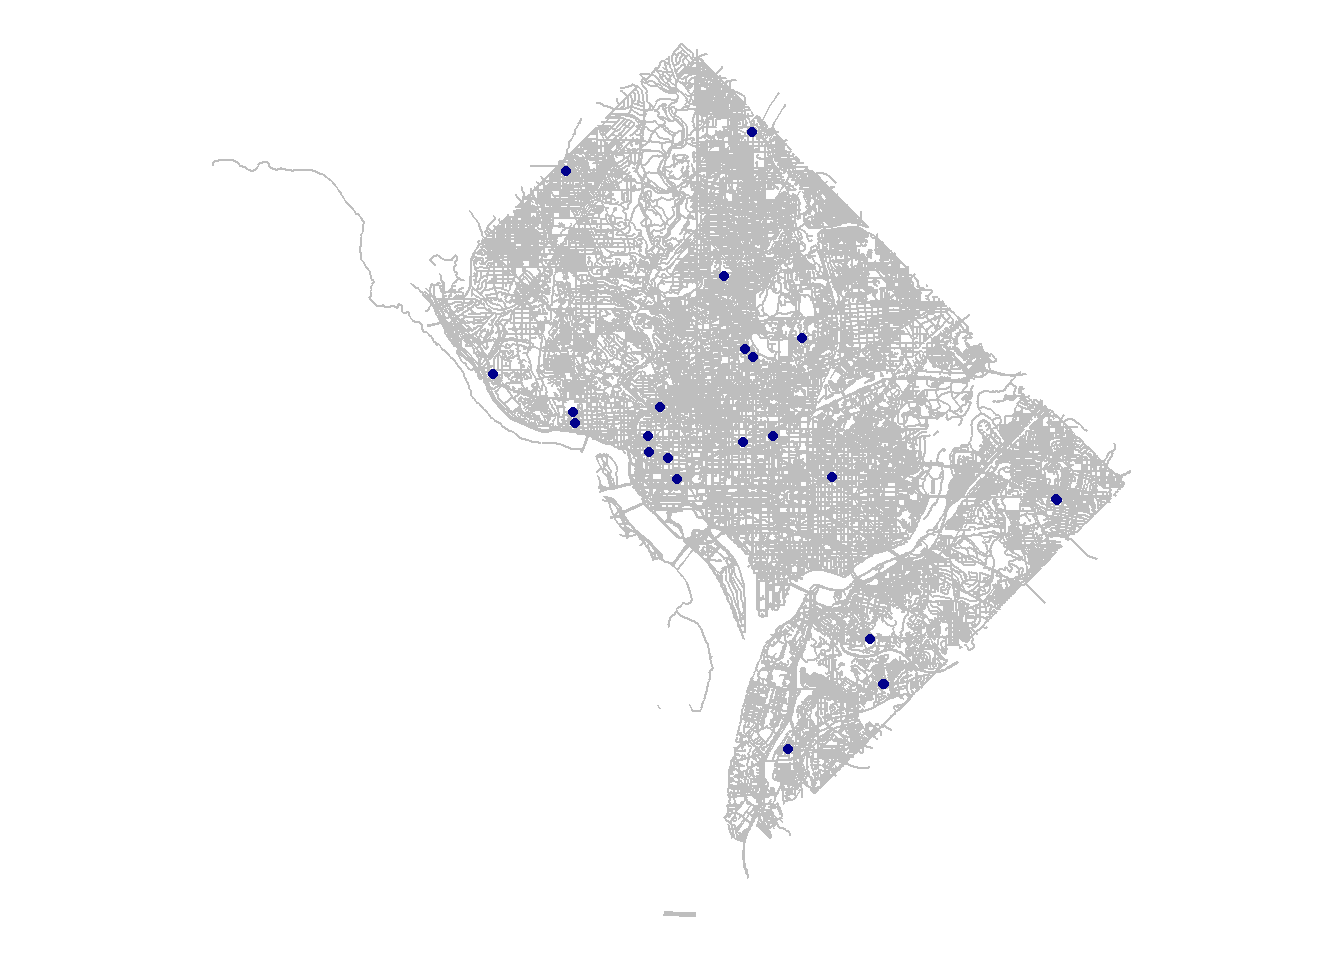
\includegraphics{Networks1_files/figure-latex/unnamed-chunk-7-1.pdf}

\begin{Shaded}
\begin{Highlighting}[]
\NormalTok{grid }\OtherTok{\textless{}{-}} \FunctionTok{st\_sf}\NormalTok{(}\FunctionTok{st\_make\_grid}\NormalTok{(DC\_city\_limits, }
                           \AttributeTok{square =} \ConstantTok{FALSE}\NormalTok{, }
                           \AttributeTok{n =} \FunctionTok{c}\NormalTok{(}\DecValTok{100}\NormalTok{,}\DecValTok{100}\NormalTok{),}
                           \AttributeTok{what =} \StringTok{"polygons"}\NormalTok{)) }\SpecialCharTok{\%\textgreater{}\%}
  \FunctionTok{st\_filter}\NormalTok{(DC\_city\_limits) }

\FunctionTok{colnames}\NormalTok{(grid) }\OtherTok{\textless{}{-}} \StringTok{"geometry"}
\FunctionTok{st\_geometry}\NormalTok{(grid) }\OtherTok{\textless{}{-}} \StringTok{"geometry"}

\NormalTok{grid }\OtherTok{\textless{}{-}}\NormalTok{ grid }\SpecialCharTok{\%\textgreater{}\%}
  \FunctionTok{mutate}\NormalTok{(}\AttributeTok{id =} \FunctionTok{seq}\NormalTok{(}\DecValTok{1}\NormalTok{, }\FunctionTok{length}\NormalTok{(grid}\SpecialCharTok{$}\NormalTok{geometry), }\AttributeTok{by=}\DecValTok{1}\NormalTok{))}

\NormalTok{grid\_points }\OtherTok{\textless{}{-}} \FunctionTok{st\_centroid}\NormalTok{(grid)}
\end{Highlighting}
\end{Shaded}

\begin{verbatim}
## Warning in st_centroid.sf(grid): st_centroid assumes attributes are constant
## over geometries of x
\end{verbatim}

\begin{Shaded}
\begin{Highlighting}[]
\FunctionTok{ggplot}\NormalTok{(grid) }\SpecialCharTok{+}
  \FunctionTok{geom\_sf}\NormalTok{() }\SpecialCharTok{+}
  \FunctionTok{geom\_sf}\NormalTok{(}\AttributeTok{data =}\NormalTok{ DC\_libraries, }\AttributeTok{color =} \StringTok{"darkblue"}\NormalTok{) }\SpecialCharTok{+}
  \FunctionTok{geom\_sf}\NormalTok{(}\AttributeTok{data =}\NormalTok{ DC\_streets, }\AttributeTok{alpha =} \FloatTok{0.2}\NormalTok{) }\SpecialCharTok{+}
  \FunctionTok{coord\_sf}\NormalTok{(}\AttributeTok{crs =}\NormalTok{ MD\_state\_plane) }\SpecialCharTok{+} 
  \FunctionTok{theme\_map}\NormalTok{()}
\end{Highlighting}
\end{Shaded}

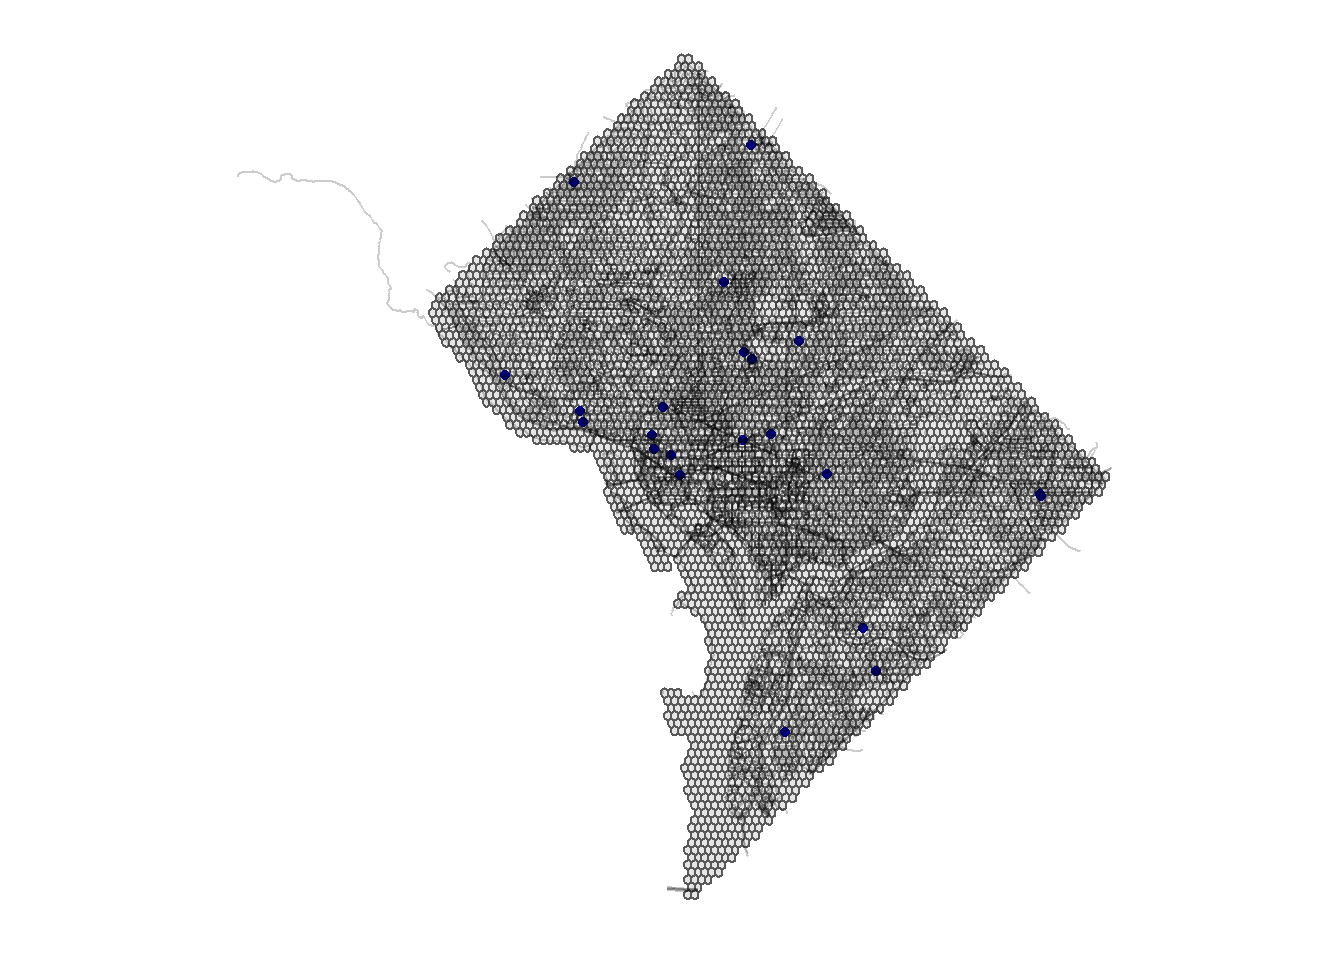
\includegraphics{Networks1_files/figure-latex/unnamed-chunk-8-1.pdf}

\begin{Shaded}
\begin{Highlighting}[]
\NormalTok{r5r\_core }\OtherTok{\textless{}{-}} \FunctionTok{setup\_r5}\NormalTok{(}\StringTok{"networks"}\NormalTok{, }\AttributeTok{verbose =} \ConstantTok{FALSE}\NormalTok{)}
\end{Highlighting}
\end{Shaded}

\begin{verbatim}
## Using cached version from C:/Users/mdelo/Dropbox/My PC (DESKTOP-R1T7JTL)/Documents/R/win-library/4.1/r5r/jar/r5-v6.2-all_20210408.jar
\end{verbatim}

\begin{verbatim}
## 
## Using cached network.dat from networks/network.dat
\end{verbatim}

\begin{Shaded}
\begin{Highlighting}[]
\NormalTok{ttm }\OtherTok{\textless{}{-}} \FunctionTok{travel\_time\_matrix}\NormalTok{(}\AttributeTok{r5r\_core =}\NormalTok{ r5r\_core,}
                          \AttributeTok{origins =}\NormalTok{ DC\_libraries,}
                          \AttributeTok{destinations =}\NormalTok{ grid\_points,}
                          \AttributeTok{mode =} \FunctionTok{c}\NormalTok{(}\StringTok{"WALK"}\NormalTok{),}
                          \AttributeTok{departure\_datetime =} \FunctionTok{as.POSIXct}\NormalTok{(}\StringTok{"15{-}03{-}2020 14:00:00"}\NormalTok{,}
                                 \AttributeTok{format =} \StringTok{"\%d{-}\%m{-}\%Y \%H:\%M:\%S"}\NormalTok{),}
                          \AttributeTok{max\_walk\_dist =} \DecValTok{1000}\NormalTok{,}
                          \AttributeTok{max\_trip\_duration =} \DecValTok{480}\NormalTok{,}
                          \AttributeTok{verbose =} \ConstantTok{FALSE}\NormalTok{)}
\end{Highlighting}
\end{Shaded}

\begin{verbatim}
## Warning in assert_points_input(destinations, "destinations"): 'destinations$id'
## forcefully cast to character.
\end{verbatim}

\begin{Shaded}
\begin{Highlighting}[]
\NormalTok{tt\_wide }\OtherTok{\textless{}{-}}\NormalTok{ ttm }\SpecialCharTok{\%\textgreater{}\%}
  \FunctionTok{pivot\_wider}\NormalTok{(}\AttributeTok{names\_from =}\NormalTok{ fromId, }
              \AttributeTok{names\_prefix =} \StringTok{"from"}\NormalTok{, }\AttributeTok{values\_from =}\NormalTok{ travel\_time) }\SpecialCharTok{\%\textgreater{}\%}
  \FunctionTok{rename}\NormalTok{(}\AttributeTok{id =}\NormalTok{ toId) }\SpecialCharTok{\%\textgreater{}\%} 
  \FunctionTok{merge}\NormalTok{(grid) }\SpecialCharTok{\%\textgreater{}\%}
  \FunctionTok{replace}\NormalTok{(}\FunctionTok{is.na}\NormalTok{(.), }\DecValTok{999}\NormalTok{) }\SpecialCharTok{\%\textgreater{}\%}
  \FunctionTok{rowwise}\NormalTok{() }\SpecialCharTok{\%\textgreater{}\%}
  \FunctionTok{mutate}\NormalTok{(}\AttributeTok{from\_any =} \FunctionTok{min}\NormalTok{(}\FunctionTok{c\_across}\NormalTok{(}\FunctionTok{starts\_with}\NormalTok{(}\StringTok{"from"}\NormalTok{)), }\AttributeTok{na.rm =} \ConstantTok{TRUE}\NormalTok{))}

\FunctionTok{st\_geometry}\NormalTok{(tt\_wide) }\OtherTok{\textless{}{-}} \StringTok{"geometry"}
\end{Highlighting}
\end{Shaded}

\begin{Shaded}
\begin{Highlighting}[]
\FunctionTok{ggplot}\NormalTok{(DC\_streets) }\SpecialCharTok{+}
  \FunctionTok{geom\_sf}\NormalTok{(}\AttributeTok{data =}\NormalTok{ tt\_wide, }
          \FunctionTok{aes}\NormalTok{(}\AttributeTok{fill =}\NormalTok{ from\_any), }
          \AttributeTok{color =} \ConstantTok{NA}\NormalTok{) }\SpecialCharTok{+}
  \FunctionTok{geom\_sf}\NormalTok{(}\AttributeTok{alpha =} \FloatTok{0.1}\NormalTok{) }\SpecialCharTok{+}
  \FunctionTok{scale\_fill\_gradient2}\NormalTok{(}\AttributeTok{low =} \StringTok{"green"}\NormalTok{, }\AttributeTok{mid =} \StringTok{"yellow"}\NormalTok{, }\AttributeTok{high =} \StringTok{"red"}\NormalTok{, }
                       \AttributeTok{midpoint =} \DecValTok{30}\NormalTok{,}
        \AttributeTok{name =} \StringTok{"Transit Travel}\SpecialCharTok{\textbackslash{}n}\StringTok{time to the}\SpecialCharTok{\textbackslash{}n}\StringTok{nearest library}\SpecialCharTok{\textbackslash{}n}\StringTok{(minutes)"}\NormalTok{) }\SpecialCharTok{+}
  \FunctionTok{coord\_sf}\NormalTok{(}\AttributeTok{crs =}\NormalTok{ MD\_state\_plane) }\SpecialCharTok{+}
 \FunctionTok{geom\_sf}\NormalTok{(}\AttributeTok{data =}\NormalTok{ DC\_libraries, }\AttributeTok{color =} \StringTok{"darkblue"}\NormalTok{) }\SpecialCharTok{+}
   \FunctionTok{theme\_map}\NormalTok{()}
\end{Highlighting}
\end{Shaded}

\begin{verbatim}
## Coordinate system already present. Adding new coordinate system, which will replace the existing one.
\end{verbatim}

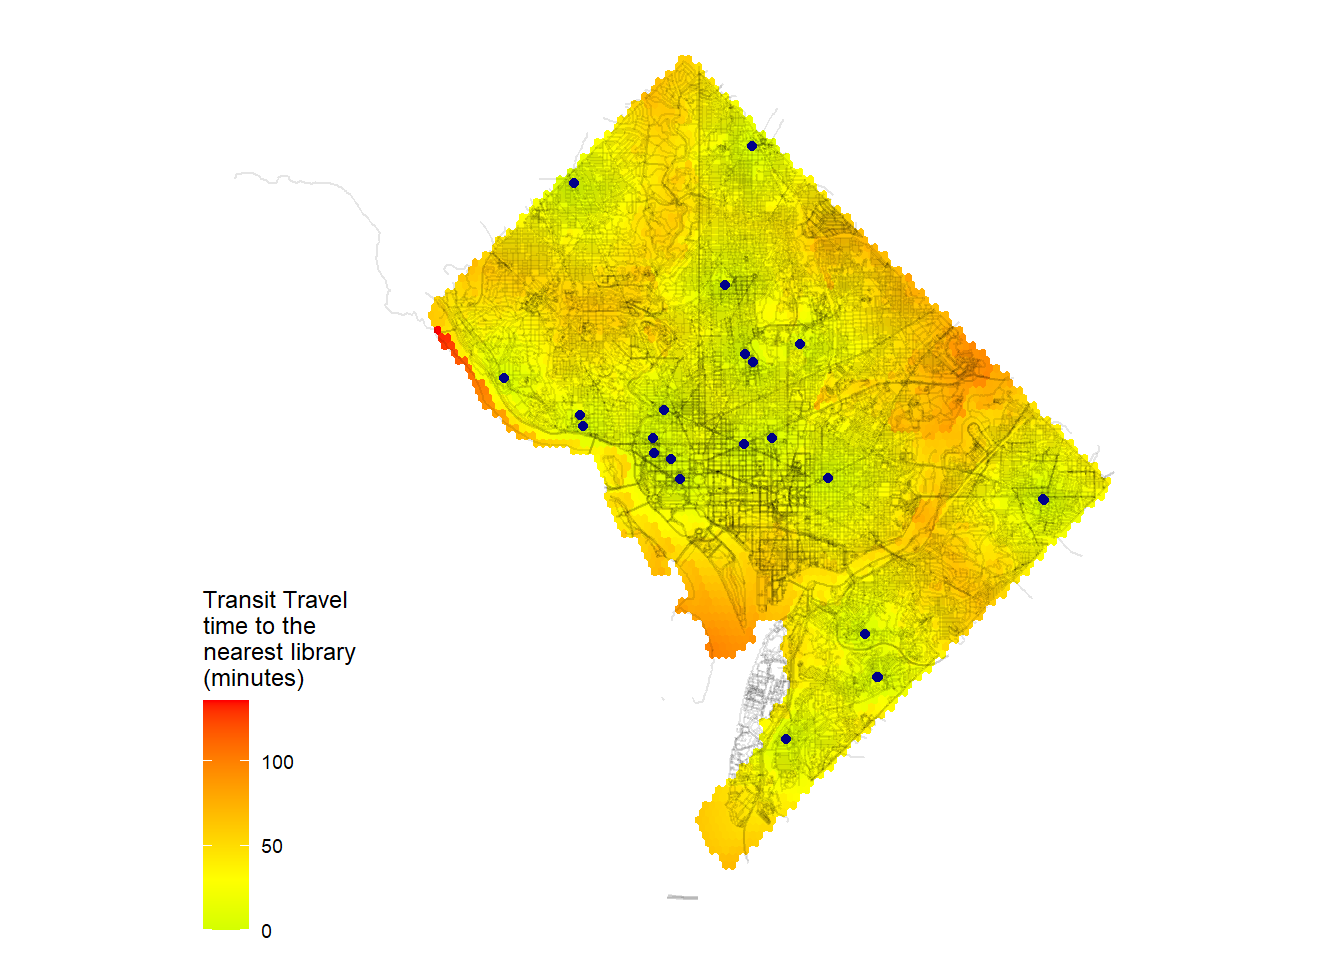
\includegraphics{Networks1_files/figure-latex/unnamed-chunk-13-1.pdf}

\begin{Shaded}
\begin{Highlighting}[]
\NormalTok{iso\_pallete }\OtherTok{\textless{}{-}} \FunctionTok{wes\_palette}\NormalTok{(}\StringTok{"Darjeeling1"}\NormalTok{, }\AttributeTok{n =} \DecValTok{5}\NormalTok{)}

\NormalTok{iso10min }\OtherTok{\textless{}{-}}\NormalTok{ tt\_wide[tt\_wide}\SpecialCharTok{$}\NormalTok{from\_any }\SpecialCharTok{\textless{}} \DecValTok{11}\NormalTok{,] }\SpecialCharTok{\%\textgreater{}\%}
  \FunctionTok{st\_union}\NormalTok{()}

\NormalTok{iso20min }\OtherTok{\textless{}{-}}\NormalTok{ tt\_wide[tt\_wide}\SpecialCharTok{$}\NormalTok{from\_any }\SpecialCharTok{\textless{}} \DecValTok{21}\NormalTok{,] }\SpecialCharTok{\%\textgreater{}\%}
  \FunctionTok{st\_union}\NormalTok{()}

\NormalTok{iso30min }\OtherTok{\textless{}{-}}\NormalTok{ tt\_wide[tt\_wide}\SpecialCharTok{$}\NormalTok{from\_any }\SpecialCharTok{\textless{}} \DecValTok{31}\NormalTok{,] }\SpecialCharTok{\%\textgreater{}\%}
  \FunctionTok{st\_union}\NormalTok{()}

\NormalTok{iso40min }\OtherTok{\textless{}{-}}\NormalTok{ tt\_wide[tt\_wide}\SpecialCharTok{$}\NormalTok{from\_any }\SpecialCharTok{\textless{}} \DecValTok{41}\NormalTok{,] }\SpecialCharTok{\%\textgreater{}\%}
  \FunctionTok{st\_union}\NormalTok{()}

\NormalTok{iso50min }\OtherTok{\textless{}{-}}\NormalTok{ tt\_wide[tt\_wide}\SpecialCharTok{$}\NormalTok{from\_any }\SpecialCharTok{\textless{}} \DecValTok{51}\NormalTok{,] }\SpecialCharTok{\%\textgreater{}\%}
  \FunctionTok{st\_union}\NormalTok{()}

\FunctionTok{ggplot}\NormalTok{(DC\_streets) }\SpecialCharTok{+}
  \FunctionTok{geom\_sf}\NormalTok{(}\AttributeTok{data =}\NormalTok{ iso50min, }
          \FunctionTok{aes}\NormalTok{(}\AttributeTok{fill =} \StringTok{"Area within 50 minutes"}\NormalTok{), }
          \AttributeTok{color =} \ConstantTok{NA}\NormalTok{) }\SpecialCharTok{+}  
  \FunctionTok{geom\_sf}\NormalTok{(}\AttributeTok{data =}\NormalTok{ iso40min, }
          \FunctionTok{aes}\NormalTok{(}\AttributeTok{fill =} \StringTok{"Area within 40 minutes"}\NormalTok{), }
          \AttributeTok{color =} \ConstantTok{NA}\NormalTok{) }\SpecialCharTok{+}
  \FunctionTok{geom\_sf}\NormalTok{(}\AttributeTok{data =}\NormalTok{ iso30min, }
          \FunctionTok{aes}\NormalTok{(}\AttributeTok{fill =} \StringTok{"Area within 30 minutes"}\NormalTok{), }
          \AttributeTok{color =} \ConstantTok{NA}\NormalTok{) }\SpecialCharTok{+}
  \FunctionTok{geom\_sf}\NormalTok{(}\AttributeTok{data =}\NormalTok{ iso20min, }
          \FunctionTok{aes}\NormalTok{(}\AttributeTok{fill =} \StringTok{"Area within 20 minutes"}\NormalTok{), }
          \AttributeTok{color =} \ConstantTok{NA}\NormalTok{) }\SpecialCharTok{+}
  \FunctionTok{geom\_sf}\NormalTok{(}\AttributeTok{data =}\NormalTok{ iso10min, }
          \FunctionTok{aes}\NormalTok{(}\AttributeTok{fill =} \StringTok{"Area within 10 minutes"}\NormalTok{), }
          \AttributeTok{color =} \ConstantTok{NA}\NormalTok{) }\SpecialCharTok{+}
  \FunctionTok{geom\_sf}\NormalTok{(}\AttributeTok{alpha =} \FloatTok{0.1}\NormalTok{) }\SpecialCharTok{+}
  \FunctionTok{scale\_fill\_manual}\NormalTok{(}\AttributeTok{values =} \FunctionTok{c}\NormalTok{(iso\_pallete[}\DecValTok{1}\NormalTok{],}
\NormalTok{                               iso\_pallete[}\DecValTok{2}\NormalTok{],}
\NormalTok{                               iso\_pallete[}\DecValTok{3}\NormalTok{],}
\NormalTok{                               iso\_pallete[}\DecValTok{4}\NormalTok{],}
\NormalTok{                               iso\_pallete[}\DecValTok{5}\NormalTok{]),}
        \AttributeTok{name =} \StringTok{"Transit Travel}\SpecialCharTok{\textbackslash{}n}\StringTok{time to the}\SpecialCharTok{\textbackslash{}n}\StringTok{nearest library}\SpecialCharTok{\textbackslash{}n}\StringTok{(minutes)"}\NormalTok{) }\SpecialCharTok{+}
  \FunctionTok{coord\_sf}\NormalTok{(}\AttributeTok{crs =}\NormalTok{ MD\_state\_plane) }\SpecialCharTok{+}
  \FunctionTok{theme\_map}\NormalTok{()}
\end{Highlighting}
\end{Shaded}

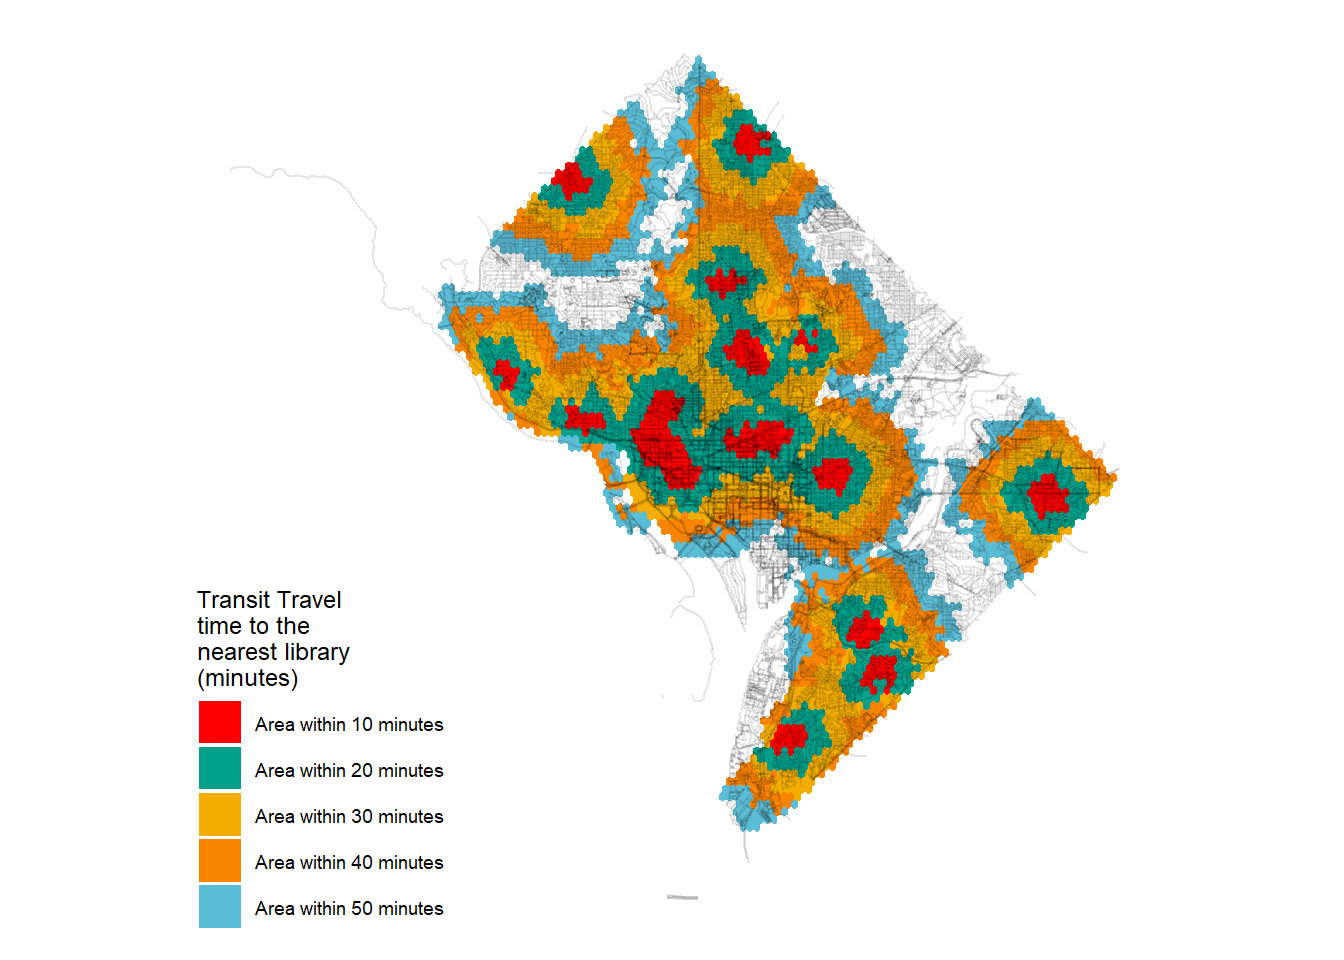
\includegraphics{Networks1_files/figure-latex/unnamed-chunk-14-1.pdf}

\begin{Shaded}
\begin{Highlighting}[]
\NormalTok{DC\_transit }\OtherTok{\textless{}{-}} \FunctionTok{read\_gtfs}\NormalTok{(}\FunctionTok{file.path}\NormalTok{(}\StringTok{"networks"}\NormalTok{, }\StringTok{"DCgtfs.zip"}\NormalTok{))}
\end{Highlighting}
\end{Shaded}

\begin{verbatim}
## Warning in set_dates_services(g): No valid dates defined in feed
\end{verbatim}

\begin{Shaded}
\begin{Highlighting}[]
\NormalTok{transit\_stops }\OtherTok{\textless{}{-}} \FunctionTok{st\_as\_sf}\NormalTok{(DC\_transit}\SpecialCharTok{$}\NormalTok{stops, }
                          \AttributeTok{coords =} \FunctionTok{c}\NormalTok{(}\StringTok{"stop\_lon"}\NormalTok{, }\StringTok{"stop\_lat"}\NormalTok{), }
                          \AttributeTok{crs =}\FunctionTok{st\_crs}\NormalTok{(grid))}
\end{Highlighting}
\end{Shaded}

\begin{Shaded}
\begin{Highlighting}[]
\NormalTok{transit\_grid }\OtherTok{\textless{}{-}}\NormalTok{ grid }\SpecialCharTok{\%\textgreater{}\%}
  \FunctionTok{mutate}\NormalTok{(}\AttributeTok{num\_stops =} \FunctionTok{lengths}\NormalTok{(}\FunctionTok{st\_covers}\NormalTok{(grid, transit\_stops)))}

\NormalTok{transit\_points }\OtherTok{\textless{}{-}} \FunctionTok{st\_centroid}\NormalTok{(transit\_grid)}
\end{Highlighting}
\end{Shaded}

\begin{verbatim}
## Warning in st_centroid.sf(transit_grid): st_centroid assumes attributes are
## constant over geometries of x
\end{verbatim}

\begin{Shaded}
\begin{Highlighting}[]
\FunctionTok{ggplot}\NormalTok{(transit\_points) }\SpecialCharTok{+}
  \FunctionTok{geom\_sf}\NormalTok{(}\FunctionTok{aes}\NormalTok{(}\AttributeTok{color =} \FunctionTok{as.character}\NormalTok{(num\_stops))) }\SpecialCharTok{+}
  \FunctionTok{scale\_color\_manual}\NormalTok{(}\AttributeTok{values =} \FunctionTok{c}\NormalTok{(}\StringTok{"gray"}\NormalTok{, }\StringTok{"cornsilk"}\NormalTok{, }\StringTok{"lightgreen"}\NormalTok{, }\StringTok{"darkgreen"}\NormalTok{, }\StringTok{"coral2"}\NormalTok{, }\StringTok{"aquamarine1"}\NormalTok{, }\StringTok{"cornflowerblue"}\NormalTok{, }\StringTok{"cyan"}\NormalTok{, }\StringTok{"darkorchid"}\NormalTok{, }\StringTok{"goldenrod"}\NormalTok{, }\StringTok{"darkorange"}\NormalTok{, }\StringTok{"deeppink"}\NormalTok{), }
                    \AttributeTok{name =} \StringTok{"Number of}\SpecialCharTok{\textbackslash{}n}\StringTok{transit stops"}\NormalTok{) }\SpecialCharTok{+}
  \FunctionTok{theme\_void}\NormalTok{()}
\end{Highlighting}
\end{Shaded}

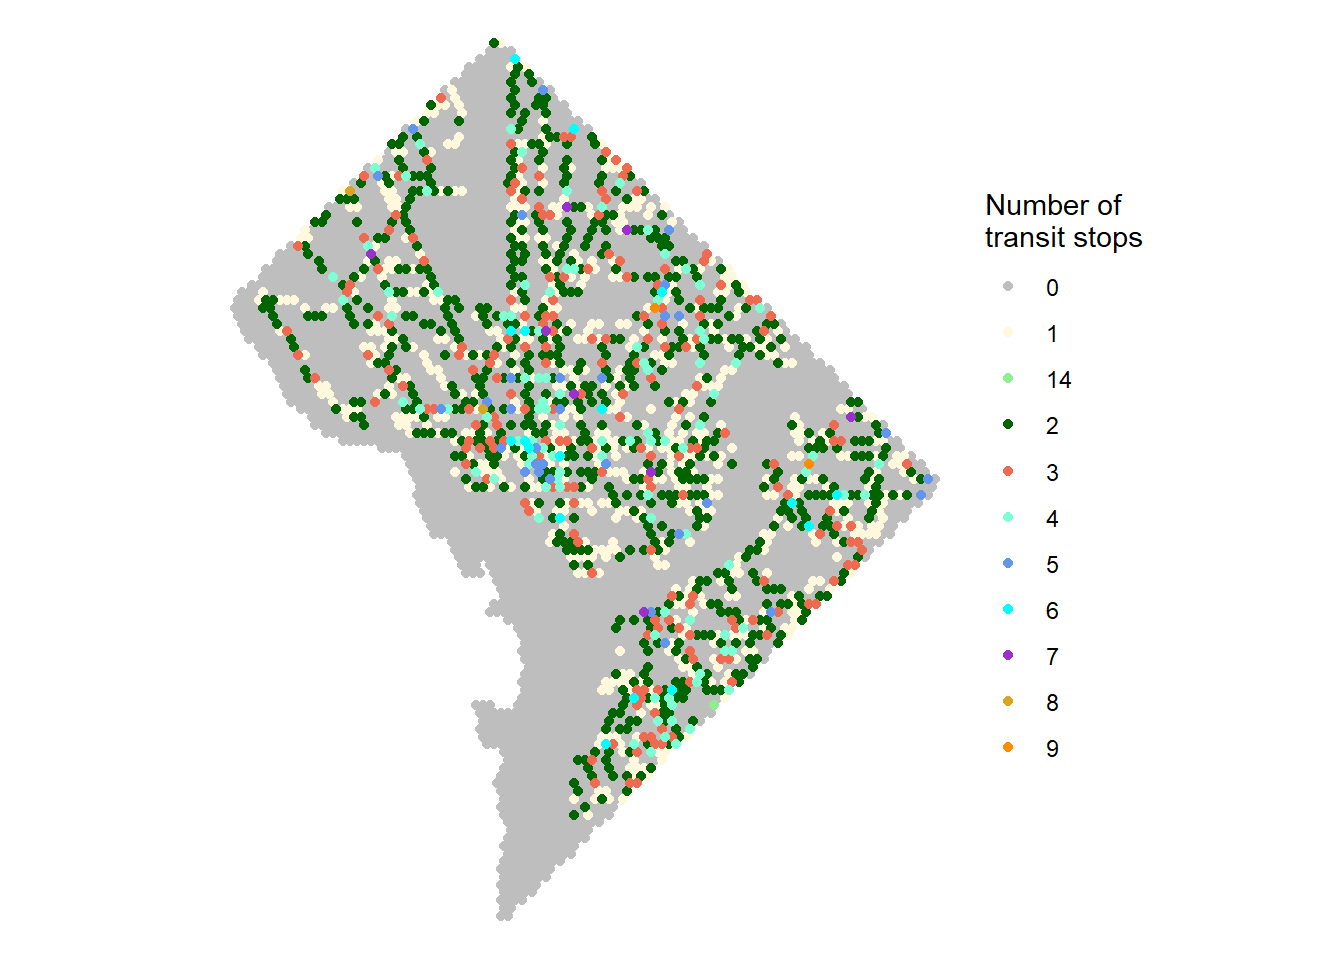
\includegraphics{Networks1_files/figure-latex/unnamed-chunk-16-1.pdf}

\begin{Shaded}
\begin{Highlighting}[]
\NormalTok{transit\_access }\OtherTok{\textless{}{-}} \FunctionTok{accessibility}\NormalTok{(r5r\_core,}
                        \AttributeTok{origins =}\NormalTok{ transit\_points,}
                        \AttributeTok{destinations =}\NormalTok{ transit\_points,}
                        \AttributeTok{mode =} \StringTok{"WALK"}\NormalTok{,}
                        \AttributeTok{opportunities\_colname =} \StringTok{"num\_stops"}\NormalTok{,}
                        \AttributeTok{decay\_function =} \StringTok{"step"}\NormalTok{,}
                        \AttributeTok{cutoffs =} \DecValTok{6}\NormalTok{,}
                        \AttributeTok{departure\_datetime =} \FunctionTok{as.POSIXct}\NormalTok{(}\StringTok{"15{-}03{-}2020 14:00:00"}\NormalTok{,}
                                 \AttributeTok{format =} \StringTok{"\%d{-}\%m{-}\%Y \%H:\%M:\%S"}\NormalTok{),}
                        \AttributeTok{max\_walk\_dist =} \DecValTok{500}\NormalTok{,}
                        \AttributeTok{time\_window =} \DecValTok{60}\NormalTok{,}
                        \AttributeTok{percentiles =} \DecValTok{50}\NormalTok{,}
                        \AttributeTok{verbose =} \ConstantTok{FALSE}\NormalTok{) }\SpecialCharTok{\%\textgreater{}\%}
  \FunctionTok{mutate}\NormalTok{(}\AttributeTok{id =} \FunctionTok{as.numeric}\NormalTok{(from\_id)) }\SpecialCharTok{\%\textgreater{}\%}
  \FunctionTok{merge}\NormalTok{(grid)}
\end{Highlighting}
\end{Shaded}

\begin{verbatim}
## Warning in assert_points_input(origins, "origins"): 'origins$id' forcefully cast
## to character.
\end{verbatim}

\begin{verbatim}
## Warning in assert_points_input(destinations, "destinations"): 'destinations$id'
## forcefully cast to character.
\end{verbatim}

\begin{Shaded}
\begin{Highlighting}[]
\FunctionTok{st\_geometry}\NormalTok{(transit\_access) }\OtherTok{\textless{}{-}} \StringTok{"geometry"}

\FunctionTok{ggplot}\NormalTok{(transit\_access) }\SpecialCharTok{+}
  \FunctionTok{geom\_sf}\NormalTok{(}\FunctionTok{aes}\NormalTok{(}\AttributeTok{fill =}\NormalTok{ accessibility), }\AttributeTok{color =} \ConstantTok{NA}\NormalTok{) }\SpecialCharTok{+}
  \FunctionTok{scale\_fill\_viridis\_c}\NormalTok{(}\AttributeTok{name =} \StringTok{"Transit stops}\SpecialCharTok{\textbackslash{}n}\StringTok{within 5{-}minutes}\SpecialCharTok{\textbackslash{}n}\StringTok{walk"}\NormalTok{) }\SpecialCharTok{+}
  \FunctionTok{coord\_sf}\NormalTok{(}\AttributeTok{crs =}\NormalTok{ MD\_state\_plane) }\SpecialCharTok{+}
  \FunctionTok{theme\_void}\NormalTok{()}
\end{Highlighting}
\end{Shaded}

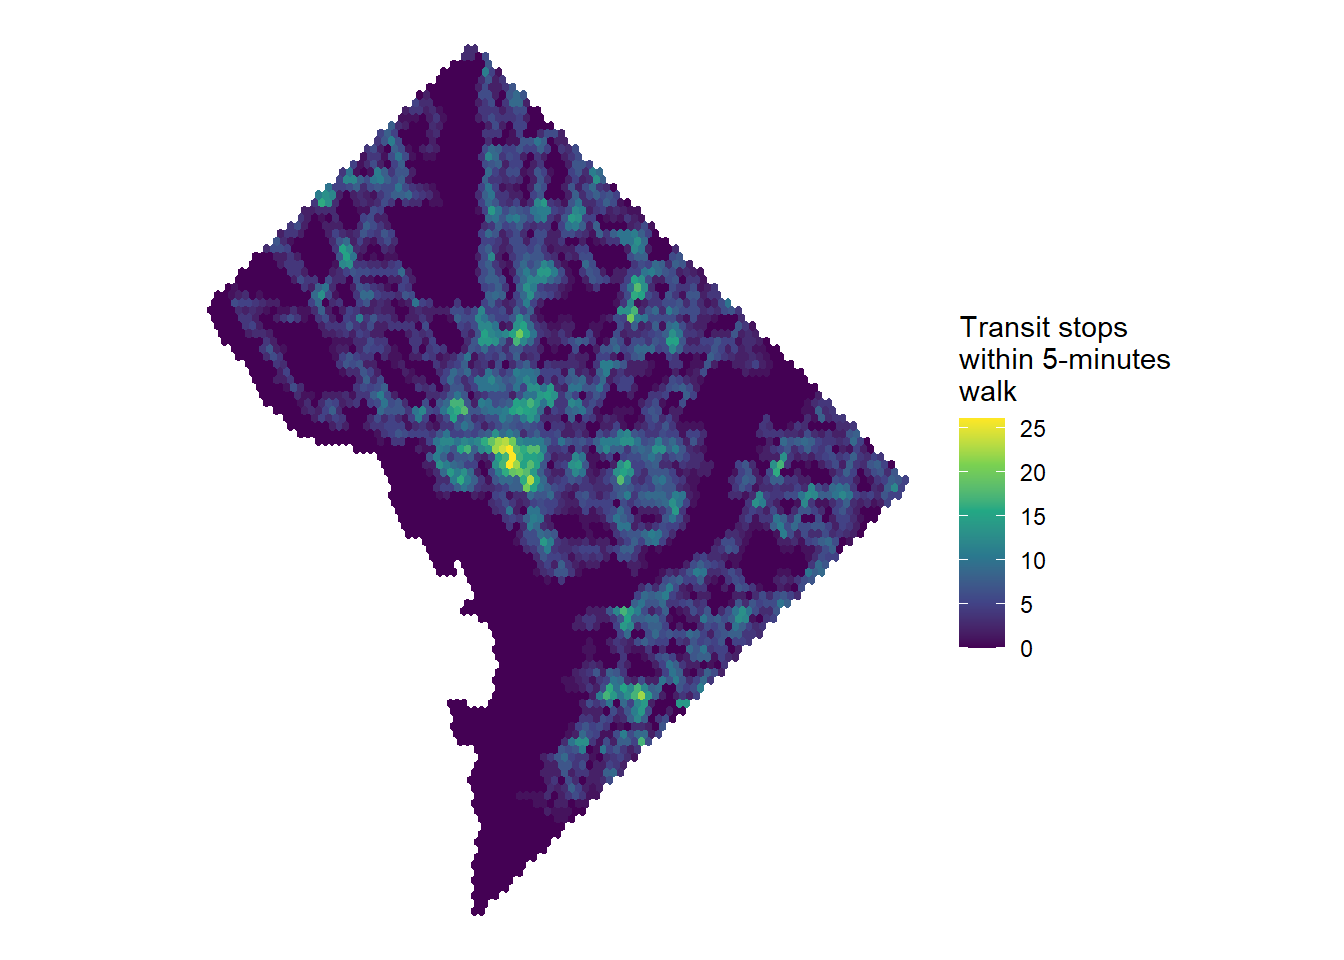
\includegraphics{Networks1_files/figure-latex/unnamed-chunk-17-1.pdf}

\begin{Shaded}
\begin{Highlighting}[]
\NormalTok{transit\_access2 }\OtherTok{\textless{}{-}} \FunctionTok{accessibility}\NormalTok{(r5r\_core,}
                        \AttributeTok{origins =}\NormalTok{ transit\_points,}
                        \AttributeTok{destinations =}\NormalTok{ transit\_points,}
                        \AttributeTok{mode =} \StringTok{"WALK"}\NormalTok{,}
                        \AttributeTok{opportunities\_colname =} \StringTok{"num\_stops"}\NormalTok{,}
                        \AttributeTok{decay\_function =} \StringTok{"exponential"}\NormalTok{,}
                        \AttributeTok{cutoffs =} \DecValTok{5}\NormalTok{,}
                        \AttributeTok{departure\_datetime =} \FunctionTok{as.POSIXct}\NormalTok{(}\StringTok{"15{-}03{-}2020 14:00:00"}\NormalTok{,}
                                 \AttributeTok{format =} \StringTok{"\%d{-}\%m{-}\%Y \%H:\%M:\%S"}\NormalTok{),}
                        \AttributeTok{max\_walk\_dist =} \DecValTok{500}\NormalTok{,}
                        \AttributeTok{time\_window =} \DecValTok{60}\NormalTok{,}
                        \AttributeTok{percentiles =} \DecValTok{50}\NormalTok{,}
                        \AttributeTok{verbose =} \ConstantTok{FALSE}\NormalTok{) }\SpecialCharTok{\%\textgreater{}\%}
  \FunctionTok{mutate}\NormalTok{(}\AttributeTok{id =} \FunctionTok{as.numeric}\NormalTok{(from\_id)) }\SpecialCharTok{\%\textgreater{}\%}
  \FunctionTok{merge}\NormalTok{(grid)}
\end{Highlighting}
\end{Shaded}

\begin{verbatim}
## Warning in assert_points_input(origins, "origins"): 'origins$id' forcefully cast
## to character.
\end{verbatim}

\begin{verbatim}
## Warning in assert_points_input(destinations, "destinations"): 'destinations$id'
## forcefully cast to character.
\end{verbatim}

\begin{Shaded}
\begin{Highlighting}[]
\FunctionTok{st\_geometry}\NormalTok{(transit\_access2) }\OtherTok{\textless{}{-}} \StringTok{"geometry"}

\FunctionTok{ggplot}\NormalTok{(transit\_access2) }\SpecialCharTok{+}
  \FunctionTok{geom\_sf}\NormalTok{(}\FunctionTok{aes}\NormalTok{(}\AttributeTok{fill =}\NormalTok{ accessibility), }\AttributeTok{color =} \ConstantTok{NA}\NormalTok{) }\SpecialCharTok{+}
  \FunctionTok{scale\_fill\_viridis\_c}\NormalTok{( }\AttributeTok{name =} \StringTok{"Accessiblity score"}\NormalTok{) }\SpecialCharTok{+}
  \FunctionTok{coord\_sf}\NormalTok{(}\AttributeTok{crs =}\NormalTok{ MD\_state\_plane) }\SpecialCharTok{+}
  \FunctionTok{theme\_void}\NormalTok{()}
\end{Highlighting}
\end{Shaded}

\includegraphics{Networks1_files/figure-latex/unnamed-chunk-18-1.pdf}

\begin{Shaded}
\begin{Highlighting}[]
\FunctionTok{stop\_r5}\NormalTok{(r5r\_core)}
\end{Highlighting}
\end{Shaded}

\begin{verbatim}
## r5r_core has been successfully stopped.
\end{verbatim}

\begin{Shaded}
\begin{Highlighting}[]
\NormalTok{rJava}\SpecialCharTok{::}\FunctionTok{.jgc}\NormalTok{(}\AttributeTok{R.gc =} \ConstantTok{TRUE}\NormalTok{)}
\end{Highlighting}
\end{Shaded}

\begin{Shaded}
\begin{Highlighting}[]
\FunctionTok{st\_write}\NormalTok{(transit\_access2, }\StringTok{\textquotesingle{}DC\_access.geojson\textquotesingle{}}\NormalTok{, }\AttributeTok{append=}\ConstantTok{FALSE}\NormalTok{, }\AttributeTok{quiet=}\ConstantTok{TRUE}\NormalTok{ )}
\end{Highlighting}
\end{Shaded}

\begin{verbatim}
## Warning in CPL_write_ogr(obj, dsn, layer, driver,
## as.character(dataset_options), : GDAL Error 6: DeleteLayer() not supported by
## this dataset.
\end{verbatim}

\end{document}
